\documentclass[a4paper,oneside,12pt]{book}
%\documentclass[numbered,print,index]{Classes/PhDThesisPSnPDF}
\usepackage{helvet}
\renewcommand{\familydefault}{\sfdefault}

\RequirePackage[intoc]{nomencl}
\makenomenclature
\renewcommand{\nomgroup}[1]{%
\ifthenelse{\equal{#1}{K}}{\item[\textbf{Key Concepts and Phrases}]}{%
\ifthenelse{\equal{#1}{A}}{\item[\textbf{Roman Symbols}]}{%
\ifthenelse{\equal{#1}{G}}{\item[\textbf{Greek Symbols}]}{%
\ifthenelse{\equal{#1}{Z}}{\item[\textbf{Acronyms / Abbreviations}]}{%
\ifthenelse{\equal{#1}{R}}{\item[\textbf{Superscripts}]}{%
\ifthenelse{\equal{#1}{S}}{\item[\textbf{Subscripts}]}{%
\ifthenelse{\equal{#1}{X}}{\item[\textbf{Other Symbols}]}
{}
}% matches mathematical symbols > X
}% matches Subscripts           > S
}% matches Superscripts         > R
}% matches Abbreviations        > Z
}% matches Greek Symbols        > G
}% matches Roman Symbols        > A
}% matches Key Words and Phrases        > K

% To add nomenclature in the header
\renewcommand{\nompreamble}{\markboth{\nomname}{\nomname}}

% Add nomenclature to contents and print out nomenclature
\newcommand{\printnomencl}[1][]{
\ifthenelse{\equal {#1}{}}
{\printnomenclature}
{\printnomenclature[#1]}
%\addcontentsline{toc}{chapter}{\nomname}
}

%----------------------------------------------------------------------------------------
%	README!
%   Welcome. It's worth having a read through this file
%   to set up the broad parameters, such as the name of
%   the degree, the school/department, the type of work
%   (dissertation/Final Year Project/report, etc. as well
%   as your own details.
%----------------------------------------------------------------------------------------

%----------------------------------------------------------------------------------------
%	COVER PAGE
%   The cover page is laid out in title/title.tex. You can choose a colour
%   or black and white logo
%----------------------------------------------------------------------------------------

%----------------------------------------------------------------------------------------
%	THESIS INFORMATION
%   Put title, author name, degree, type of work, school, department in here
%   It will be used for the title page and for the embedded PDF information
%----------------------------------------------------------------------------------------

\newcommand{\thesistitle}{Title of Work} % Your thesis title, this is used in the title and abstract
\newcommand{\degree}{PhD Electronic and Electrical Engineering} % Your degree name, this is used in the title page and abstract
\newcommand{\typeofthesis}{dissertation} % dissertation, Final Year Project, report, etc.
\newcommand{\authorname}{Edward Storey} % Your name, this is used in the title page and PDF stuff
%% Do not put your Student ID in the document, as TCD will not publish
%% documents that contain both your name and your Student ID.

\newcommand{\keywords}{this, that, more} % Keywords for your thesis
\newcommand{\school}{\href{https://www.tcd.ie/Engineering/}{School of Engineering}} % Your school's name and URL, this is used in the title page
%Edited by HS for engineering

%% Comment out the next line if you don't want a department to appear
\newcommand{\department}{\href{http://researchgroup.university.com}{Sigmedia Research Lab}} % Your research group's name and URL, this is used in the title page

\AtBeginDocument{
\hypersetup{pdftitle=\thesistitle} % Set the PDF's title to your title
\hypersetup{pdfauthor=\authorname} % Set the PDF's author to your name
\hypersetup{pdfkeywords=\keywords} % Set the PDF's keywords to your keywords
\hypersetup{pdfsubject=\degree} % Set the PDF's keywords to your keywords
}

%% Johanna's note stuff
%\usepackage[colorinlistoftodos,prependcaption,textsize=tiny]{todonotes}

%% Language and font encodings
\usepackage[T1]{fontenc} 
\usepackage[utf8]{inputenc}
\usepackage[english]{babel}

%% Custom enumeration
\usepackage{enumerate}
\usepackage[shortlabels]{enumitem}

%% Bibliographical stuff
%\usepackage[round,sort,comma,numbers]{natbib}
%above commented out by HS to get [X] references instead of (X)
\usepackage[]{cite}
%% Document size
% include showframe as an option if you want to see the boxes
\usepackage[a4paper,top=2.54cm,bottom=2.54cm,left=2.54cm,right=2.54cm,headheight=16pt]{geometry}
\setlength{\marginparwidth}{2cm}
%% Useful packages
\usepackage{amsmath}
\usepackage[autostyle=true]{csquotes} % Required to generate language-dependent quotes in the bibliography
\usepackage[pdftex]{graphicx}
%\usepackage[colorinlistoftodos]{todonotes}
\usepackage[colorlinks=true, allcolors=black]{hyperref}
\usepackage{caption} % if no caption, no colon
\usepackage{sfmath} %use sans-serif in the maths sections too
\usepackage[parfill]{parskip}    % Begin paragraphs with an empty line rather than an indent
\usepackage{setspace} % to permit one-and-a-half or double spacing
\usepackage{enumerate} % fancy enumerations like (i) (ii) or (a) (b) and suchlike
\usepackage{booktabs} % To thicken table lines
\usepackage{fancyhdr}
\numberwithin{equation}{chapter} %HS edit for (chapter.equation)
\pagestyle{plain} % Embrace simplicity!

\usepackage{graphicx}% this is for rotating the plots
%\usepackage{fontspec}
\usepackage[pdftex,dvipsnames]{xcolor}
\usepackage{xargs}
\usepackage[colorinlistoftodos,prependcaption,textsize=tiny]{todonotes}
%% Johanna's extra todo stuff
\newcommandx{\thiswillnotshow}[2][1=]{\todo[disable,#1]{#2}}
\newcommandx{\unsure}[2][1=]{\todo[linecolor=yellow,backgroundcolor=yellow!25,bordercolor=yellow,#1]{#2}}
\newcommandx{\change}[2][1=]{\todo[linecolor=red,backgroundcolor=red!25,bordercolor=red,#1]{#2}}
\newcommandx{\info}[2][1=]{\todo[linecolor=gray,backgroundcolor=gray!25,bordercolor=gray,#1]{#2}}
\newcommandx{\improvement}[2][1=]{\todo[linecolor=Plum,backgroundcolor=Plum!25,bordercolor=Plum,#1]{#2}}
\newcommandx{\thoughts}[2][1=]{\todo[linecolor=purple,backgroundcolor=purple!25,bordercolor=purple,#1]{#2}}
\newcommandx{\naominote}[2][1=]{\todo[linecolor=red,backgroundcolor=yellow!25,bordercolor=red,#1]{#2}}
\newcommandx{\delphinenote}[2][1=]{\todo[linecolor=red,backgroundcolor=Plum!25,bordercolor=red,#1]{#2}}
\newcommandx{\perplexnote}[2][1=]{\todo[linecolor=OliveGreen,backgroundcolor=gray!40,bordercolor=OliveGreen,#1]{#2}}
\newcommandx{\summary}[2][1=]{\todo[linecolor=OliveGreen,backgroundcolor=green!60,bordercolor=OliveGreen,#1]{#2}}
\newcommandx{\unexplained}[2][1=]{\todo[linecolor=yellow,backgroundcolor=Plum!25,bordercolor=yellow,#1]{#2}}

\usepackage{soul}

\usepackage{tipa}
\usepackage{array}
\usepackage{longtable}
\usepackage{booktabs}
%\usepackage[margin=1in]{geometry}
%\usepackage[margin=1in]{geometry}

\usepackage{float} %% for full page figures





%% The Mechanical engineers require your name and ID on the top of every page.
%% Uncomment the following block if you want your name and ID at the top of
%% (almost) every page.

%\pagestyle{fancy}
%\fancyhf{} % sets both header and footer to nothing
%\renewcommand{\headrulewidth}{0pt}
%\cfoot{\thepage}
%\ifdefined\authorid
%\chead{\it \authorname\ (\authorid)}
%\else
%\chead{\it \authorname}
%\fi
%% End of block


\fancypagestyle{general}{
    \fancyhf{}
    \renewcommand{\headrulewidth}{0.25pt} %set to 0 for no line in header
    \renewcommand{\footrulewidth}{0.25pt} %set to 0 for no line in footer
    \fancyfoot[R]{Ed Storey}
    \fancyfoot[C]{\thepage}
    \fancyhead[R]{\rightmark}
    \fancyhead[L]{Chapter \thechapter}
}

%% It is not a requirement of the university that the font should be sans-serif, but
%% the Mechanical engineers require it. Comment out the following line to disable it
\renewcommand{\familydefault}{\sfdefault} %use the sans-serif font as default

%% If you're not using sans-serif, consider using Palatino instead of the LaTeX standard
%\usepackage{mathpazo} % Use the Palatino font by default if you prefer it to Computer Modern

%\renewcommand{\theequation}{\arabic{equation}} %% use continuous equation numbers
% The above commented out by HS to enable (Ch.Eq) format

%% Format Chapter headings appropriately
\usepackage{titlesec}
\titleformat{\chapter}[hang] 
{\normalfont\huge\bfseries}{\thechapter}{1cm}{} 
\usepackage{amsmath}


\usepackage{wrapfig}
% BEGIN: For IPA support
% Comment out serif override just for IPA if needed
% \renewcommand{\familydefault}{\sfdefault}

%\usepackage{fontspec}
%\setmainfont{Libertinus Serif} % or Charis SIL, Doulos SIL

% END: For IPA support


\title{\thesistitle}
\author{\authorname}

\frontmatter
\begin{document}
\input{title/title.tex}
\pagenumbering{roman}
\section*{\Huge{Declaration}}
\vspace{1cm}
I hereby declare that this \typeofthesis\ is entirely my own work and that it has not been submitted as an exercise for a degree at this or any other university.

\vspace{1cm}
I have read and I understand the plagiarism provisions in the General Regulations of the University Calendar for the current year, found at \url{http://www.tcd.ie/calendar}.
\vspace{1cm}

I have also completed the Online Tutorial on avoiding plagiarism `Ready Steady Write', located at \url{http://tcd-ie.libguides.com/plagiarism/ready-steady-write}.
\vspace{3cm}

Signed:~\rule{5cm}{0.3pt}\hfill Date:~\rule{5cm}{0.3pt}

\chapter*{Abstract}
%A short summary of the problem investigated, the approach taken and the key findings. This should not be more than around 400 words. They must be on a separate page.

In recent years, Automatic Speech Recognition (ASR) has vastly improved with the introduction of transformers and Self-supervised Learning (SSL). SSL models do the bulk of language learning in pretraining on large unlabelled datasets. These pretrained models can be fine-tuned to smaller datasets, producing impressive accuracy with minimal compute power. Early SSL models were pretrained on data from a single language, monolingual pretraining. However, it was found that if the fine-tuning language did not match the pretraining language, fine-tuned accuracy would decrease. 

To improve cross-lingual accuracy, SSL ASR models can be pretrained on multiple languages, multilingual pretraining. Pretraining on multilingual data improves downstream accuracy for mismatched and low-resource languages. However, multilingual pretraining has a trade-off. The more languages added to the pretraining data, the worse the fine-tuned accuracy becomes for a single language. 


%%%% Alterantive pargraph
This trade-off between multilingual pretraining and monolingual downstream accuracy can be offset by increasing the model size. However, increasing the model size increases the compute power required to train the model. Increasing computational costs disproportionately impact low-resource languages, for which multilingual models have the most positive effect on accuracy. Therefore, this thesis seeks to understand multilingual SSL ASR models to guide effective pretraining strategies.

We first examine how the large open-source multilingual model XLS-R stores language information. We analyse XLS-R weight distributions by identifying language-specific subnetworks through the use of the Lottery Ticket Hypothesis (LTH). We first fine-tune XLS-R to a single language and then apply unstructured pruning to find the language-specific subnetwork. We prune to increasing proportions of the model weights, in steps of 10\%, to identify the optimal network sparsity. We then repeat this process across multiple languages. We fine-tune each subnetwork to multiple languages and measure the Character Error Rate (CER). We find that XLS-R can have 50\% of its weights pruned with no increase in the CER. It can be further pruned to 70\% with only a minimal increase in CER. These findings applied to all languages tested.

We then show that the English language-specific subnetwork always produces the lowest CER when compared to subnetworks for other languages. English is the language that contains the most hours in pretraining. We therefore hypothesise that XLS-R dedicates more of its weights to English speech information than the other languages in its pretraining data. We prove this by showing that when fine-tuned to languages related to Spanish, the English language-specific subnetwork produces lower CER than the Spanish subnetwork. We also analyse the Intersection Over Union (IOU) between language-specific subnetworks. We find that the English language-specific subnetwork has the highest IOU between it and the pretrained model. We also find that the English subnetwork has a higher IOU with languages related to Spanish than the Spanish subnetwork. %This shows that XLS-R does not use information learned from related languages when performing monolingual fine-tuning. 


To further understand how this imbalance in pretraining hours affects multilingual pretraining, we next pretrain 7 of our own multilingual SSL ASR models. Of these models, 1 is a monolingual English model and 1 is a monolingual Spanish model. The  5 remaining models contain various ratios of these 2 languages. SSL pretraining only teaches phonetic features to the model, whereas semantic learning is done during fine-tuning. To test multilingual language learning, we therefore train Multi Layer Perceptrons (MLPs) on XLS-R layer outputs to probe for phoneme accuracy. 

We collect phoneme accuracy data from 4 languages: English, Spanish, French and Polish. We first test matched-language phonemes for the English and Spanish pretraining languages. We find that phoneme accuracy increases proportionally to the amount of matched language data in pretraining. We also find that for languages unseen in pretraining, French and Polish, phoneme exposure contributes to phoneme accuracy. If a phoneme is present in the pretraining data, the average accuracy for that phoneme will be higher even when spoken in an unseen, mismatched language. 

We further investigate phonetic features by grouping our phonemes into Manner of Articulation (MoA) classes. We find that MoA accuracy can also increase as the amount of matched-language data in pretraining is increased. However, how much it increases depends on the MoA class and the language it is spoken in. Class exposure in pretraining can also increase individual phoneme accuracy, even for unseen languages. However, the impact of this effect is also dependent on the MoA class. 

Finally, we suggest future work that our contributions could be applied to. We suggest multiple research directions that our contributions could be applied to in order to improve current multilingual pretraining approaches. Overall, we hope that these contributions can lead to high accuracy, low computation, multilingual SSL ASR.

\newpage
\onehalfspacing\raggedright %\raggedright turns off justification and hypenation



\section*{\Huge{Acknowledgements}}
%Thanks Mum!

%You should acknowledge any help that you have received (for example from technical staff), or input provided by, for example, a company.
\iffalse
\begin{itemize}
    \item Naomi
    \begin{itemize}
        \item Support
        \item patience through thick and thin
        \item allowed me to learn and grow
        \item That support gave me the space I needed gave me chances other people didn't
        \item I truly appreciate everything she's done for me
    \end{itemize}
    \item Sigmedia
    \begin{itemize}
        \item The old guard: DJ, Meegan, Mark, Ayushi, Sam O'C-R, Sam K, Seb, Sophia, Ciaron, Shu Darren, Clement, Vibhoothi, Shashwat, Danilo, Stephen, Arman, Justine?
        \item the new guard: Zhaofeng, Aris, Vicky, Rishabh, Delphine, Vu, Julien, Conal, Udit, Ilaria and Mel, boldo, Dee
        \item the academics
        \item the support staff
        \item maybe Fionn and disabilities can go here
    \end{itemize}
    \item Peter
    \begin{itemize}
        \item gave me a chance
        \ietm taught me a lot
    \end{itemize}
    \item Edinburgh
    \begin{itemize}
        \item Andres, Catherine, Hoa, Jason, Dan, Johanna, Sarenne
        \item thanks for the lunch break and teh very publishable ideas!
        \item I loved being in Edinburgh
    \end{itemize}
    \item D-Real
    \begin{itemize}
        \item To all and for the funding
        \item Stephen Specifically, maybe carol too
        \item a broader mention of everyone I knew from d-real
    \end{itemize}
    \item friends
    \begin{itemize}
        \item Johanna, Anna-Lisa, Rob and Lauren - All the guiness, all of the pool, all the shared PhD trauma, you guys are great
        \item Fortismere friends here?
        \item Shoutout to the York lot?
    \end{itemize}
    \item housemates
    \begin{itemize}
        \item To all the various housemates
        \item Particularly Maria and Connor
    \end{itemize}
    \item Family
    \begin{itemize}
        \item O'Driscolls? Storeys?
        \item Do I talk here about grandparents? Specifically Nana
        \item Either here or at the very end I should mention Anette
    \end{itemize}
    \item Close Family
    \item Ellie and Sam
    \item Mum and Dad
    \begin{itemize}
        \item Huge support they have always given me
        \item Particularly supportive throughout this PhD
        \item I appreciate everything they do for me and I could not have finished this PhD, or many other things, without them.
        \item I love you both and thank you.
    \end{itemize}
    \item Maybe Nana here?
    \begin{itemize}
        \item She went through a lot and did everything for her family
        \item she became a deputy head mistress because she knew what education meant for someone
        \item I wish she were here to see me graduate 
    \end{itemize}
    \item Something about Auntie Annette
    \begin{itemize}
        \item she passed too young and I miss her
        \item She was always so supportive of everything I did
        \item always so positive, always excited to ask me about my life, always so proud of me no matter what I was doing.
        \item She was a great source of support while Nana was ill and after she passed away
        \item Auntie Annette passed away just before I went to Dublin and I still miss her dearly
        \item I wish she was here to see me graduate, I will miss her over-excited hug the first time I would have seen her after graduating
        \item I can't even express how much I miss my auntie
    \end{itemize}
\end{itemize}
\fi

This PhD has been a life-changing experience for me on many levels and I wouldn't have made it this far without the help of a lot of people.

First and foremost I need to thank my supervisor Professor Naomi Harte, who gave me this chance in the first place. Naomi has stuck by me at every point of this PhD, through the lows and the highs. She is a great role model whom I have learned technically, academic and personally.\thoughts{not sure about this line, also I should say something mroe bout naomi's technical knowledge.} She was not afraid to give me the tough truth when I needed to hear it, but was also incredibly supportive when my back was up against the wall. Many people would not have gone as far as Naomi has to support me over the last few years and I will never forget that, thank you.

I must also thank Professor Peter Bell, who was my supervisor during my internship at the University of Edinburgh. Peter agreed to let me visit the informatics department in Edinburgh after I accosted him at Interspeech 2023 asking for help. He was kind and helpful and I learned a lot from his incredible knowledge of ASR. This internship led to my first publication and I will never forget that either. While I won't list them all, everyone I met at Edinburgh was also fantastic. Whether it was the great lunch chats, the weekend rugby or Johanna's great generosity of giving me a bed for my first weeks there. You all made such a difference to my time in Edinburgh, thank you.

This PhD would not have been possible without the lovely colleagues and friends I have met along the way. Professor Anil Kokaram has created a workplace that makes us all want to come in and see our colleagues every day. For that I thank him. I want to thank my Sigmedia PhD and PostDoc peers for making me look forward to work every day. To Sebastien, Mark and Ayushi and DJ who were here when I arrived. To Sophia, Ciaron, Clement, Darren, Viboothi, who started at the same time as me. To Sam O'Connor-Russel, Sam Kotey, Justine, Shashwat, Danilo, Arman, Shu and Meegan, who joined soon after. To Zhaofeng, Julien, Conal, Udit, Boldo, Sigmedia the next generation. To Aris, Vicky, Rishabh, Delphine and Vu, the most recent additions to our speech lab. To Dee, Ilaria, Mel, Stephen, whom I link simply by all being wonderful people. Whether it was what I learned from each of you, how I grew alongside you or whether you simply provided good company to enjoy a beer or a puck about. You have all made a huge impact on my life and my PhD possible, thank you. 

Additionally, to the Academics and Staff of Sigmedia, of whom I have run out of space to name. Every member of this team has been kind and patient, whilst just being excellent at each of their respective jobs. I've worked in many places and really never met a team like you. A special mention to John, who always gives me a good laugh while solving my various printer issues and Michael, who is about to enjoy a very well-deserved retirement. The Broader Trinity staff have also been excellent. Especially Fionn O'Sullivan and Declan Reilly who have been a huge part of getting me to the end, thank you.

Outside of Sigmedia I would like to thank my funding body D-Real and Professor Carol O'Sullivan who heads it. I literally would not have been to do without you. Extra thanks to Stephen Carol who was the administrator for most of my time at D-Real. He always had time to help with any minor or major issue whenever I needed anything. His organisation of writing sessions, writing retreats and various D-Real events made this PhD. More broadly I would like to thank everyone else involved with D-Real, especially the other students who made every D-Real event that much better. Thank you all.

This PhD would not have been possible without the support of my friends. I would like to thank Johanna, Anna-Lisa, Rob and Lauren, who have become lifelong friends. Every pint of Guinness, every game of pool, every brunch and day trip made me so happy, thank you so much. I'll see you all soon. I would also like to mention my friends from back home, in North London. I'm a doctor guys, none of us saw this coming! That bedrock of friendship to come back to has been so important. Wherever I was, whenever it was, you've always been such a source of strength for me and has made this PhD and many other things in my life possible, thank you. To those I met at the University of York, the place that really started this journey, thank you. A special shoutout to my old housemates, Clemmie, Lauren, Jen and Sam as well as their respective partners. As well to the various housemates I've had in Dublin, you've been great. Especially Maria and Connor who always had time for chat at the end of the day.

Briefly I would like to thank my extended family. The Storeys and O'Driscolls are made up of incredible people, who I am incredibly lucky to be related to. Every christmas gathering we do in the O'Driscoll family makes my year. It is difficult to summarise how much the O'Driscoll family means to me but, all of you, in each of your own ways, have provided such support and confort to me over the years, thank you. The Storey family are also incredible, they are inspirational, fun, smart and also supportive and mean the world to me, thank you also. I have far, far, too many family members to list by name unfortunately and it would be unfair to pick out individuals. However, I really believe that I would not be the person I am without all of you. This PhD is, in my eyes, is an achievment of our families and what makes us all special, not just me. So, thank you all, you're incredible. 

To my sister Ellie. Ellie is about to become a doctor herself having recently completed her own doctorate. Having the support of a sister who knows and understands me, has many of the same experiences and, more recently, even understands how difficult getting a doctorate is has been invaluable. Ellie is often someone I think of as just a better version of myself, she is often inspirational to me and I'm lucky to have her as a sister. Thanks sis and congratulations on your own achievement! To my soon to be brother-in-law Sam, keep doing what your doing mate. It's a joy hanging out with you when I come back to London and you have been a great support to during this time, thank you.

The most important thanks should go to my parents, Marie and Graham. My long-suffering parents have always been there for me, no matter what I was going through. They have never given up hope on me, they have always been there when I needed them and they have supported me in every decision I have ever made. For a multitude of reasons I won't list here, this PhD would in no way have been posisble without them. I love you both and don't say thank you nearly enough, for everything you do for me. So here I thank you, you mean the world to me.

\subsubsection{Those who could not be here}
I would like to set aside some space to address those who I have lost and therefore cannot be here. Firstly my Grandma Maureen, who died when I was young. I didn't get to know her well but I did see the loss that everyone felt when she went. I remember her warmth and kindness and I wish she were still here now. Grandad Dick died when I was older, but still young. He had a hard life, but never let it stop him bringing happiness to all the people around him. Sadly, the best example of this I have is his funeral, where I was amazed to see what seemed like the entirey of East London come out to mourn him. I wish I knew you both better, but I still miss you and wish you were both here now. Grandad Bob I knew a little better, he passed when I was a teenager. He was an Electrical Engineer, like me, he loved science and was proud that it was one of my favourite subjects in school. I still have the copy of Bill Bryson's "A Short History of Nearly Everything" he gave me and I sometimes read the note he wrote to me on the inside cover. I would have liked for him to have been here now to see me follow in his footsteps.

Nana Mary, my final grandparent, survived into my twenties, of all my grandparents I knew her best. Mary O'Driscoll, born Mary Burke, was a farm girl born in county Galway. She lived in a rough time in Irish history and as a young woman had to move to London to find work. There, she met my grandfather Richard [Dick] O'Driscoll. They got married and had six lovely children, the first of which was my mother Marie. Life could be hard as an Irish person in London at this time. So, after my youngest uncle was old, enough Nana would go back into the workforce. She got a job as a teacher in a local catholic shool and made her way up to deputy headmistress. This job would allowed Nana and Grandad to buy their home in Ilford. This is the home I would eventually go to visit her in many years later. Through her work and the tough times she endured, Nana had a great belief in the importance of education. It is tool to help keep her family safe and comfortable, but also a tool to help all people better understand everything and everyone around them. She passed away a few years before I moved to Ireland to study. So I can only imagine what it would have meant to her to see her grandson gradute from Trinity College Dublin. I wish she was here to see it, it would have meant the world to me. Since she isn't here, the next best thing I can do is to write about her in this thesis, for her memory to be kept on record in the Trinity Acrhives. Nana Mary, was an incredible role model for me and I think this is the least she deserves.

%Lastly I would like to remember my Auntie Annette, Annette White, born Annette O'Driscoll, who passed away a little after Nana. She passed away young from cancer and I miss her so much. Auntie Annette was always there to support me, always excited and interested in hearing about whatever I was doing at the time. She had endless positivity and joy when hearing about my life and just about anything else she talked about. 

Lastly I would like to remember my Auntie Annette, Annette White, born Annette O'Driscoll, who passed away a little after Nana. When we used to go and visit the White family in Portsmouth, I would enter the house and often be greated by the sound of Auntie Anette singing to herself in another room. She would be singing one of her favourite songs, but, as always, would have forgotten many of the words. I would walk towards the sound of her singing, I would hear her making up for the forgotten words by inserting her own additions into the song. Often she would replace the missing parts of the song with the ingredients to whatever meal she was currently preparing, such as a fruit salad. As I got closer she would see me, she would immediately stop singing about melons and apples and rush over to give me a big cuddle. She sit down and ask me endless questions about my life and be so happy with and excited about whatever answer I gave. I feel so sad when I remember that I will not be able to tell her all about my PhD graduation. To think how happy and proud she would have been and how happy that would have made me feel. I would like to share a million different stories about Auntie Annette, but after writing this I simply can't stop crying.\thoughts{probably shouldn't have this here} So, instead, I will simply send my love, and my thanks for all the years we had, to her. As well, I send my love and thanks to the whole of the White family, who have been through so much and whom I love dearly.



\tableofcontents
\listoffigures
\listoftables
\listoftodos
\printnomenclature
\newpage
%\input{Acronyms/acronyms.tex}


% ******************************* Nomenclature *********************************


\iffalse
\newpage
\section*{\Huge{Nomenclature}}
\begin{tabular}{lp{9cm}l}
A&Area of the wing&$m^{2}$\\
B\\
C& Roman letters first, with capitals\ldots\\
a&then lower case.\\
b\\
c\\
$\Gamma$&Followed by Greek capitals\ldots\\
$\alpha$&then lower case greek symbols.\\
$\beta$\\
$\epsilon$\\
TLA&Finally, three letter acronyms and other abbreviations arranged alphabetically\\
\end{tabular}
\vspace{2cm}

If a parameter has a typical unit that is used throughout your report, then it should be included here on the right hand side.

If you have a very mathematical report, then you may wish to divide the nomenclature list into functions and variables, and then sub- and super-scripts.

Note that Roman mathematical symbols are typically in a serif font in italics.
\fi

\pagestyle{general}
\mainmatter
%\printnomenclature
\chapter{Introduction}
The information contained in a single utterance of speech is vast. From only a few seconds of speech, we can identify a speaker's gender, age and their proximity relative to our own. The frequency and rhythms of speech can tell us about the urgency or the emotional weight of the statement. The harmonic nature, the placement of silence or noise and the prosody of the speech can then convey words and meaning. The pronunciation of these words can even tell us information about the speaker's region of birth or the circumstances of their upbringing. In only a few seconds, the human brain can receive and process this information-rich signal. 

From the 1950s onwards, researchers began working to achieve the automatic transcription of human speech. This is a task that, despite decades of research, has proven difficult to replicate. It is also the task that this thesis seeks to improve upon. The first step to understanding a speech signal is to compute the Fast Fourier Transform (FFT). The FFT enabled computers to decompose a speech signal into its frequency components efficiently. The FFTs for short overlapping windows of audio can then be computed and arranged over time. This produces a representation of the signal with frequency on the y axis, time on the x axis and frequency magnitude on the z axis. This representation is known as the spectrogram and allows us to visualise the breadth of information encoded in speech. 

In Figure~\ref{intro_fig:mel_spectrogram} we see an annotated mel-spectrogram of a short utterance of speech. A mel-spectrogram compresses frequency bands, giving greater resolution to lower frequencies where speech information is most concentrated. This utterance contains a speaker saying the words "which he understood". Below the spectrogram, we have marked some of the linguistic information contained in this speech sample. We see how words and characters can be represented in time and frequency. We further show how phonemes and their articulations, each of which produces observable patterns in the spectrum. The spectrogram demonstrates just how much information is transmitted through speech in only a few milliseconds (ms).

\begin{figure}[t]
    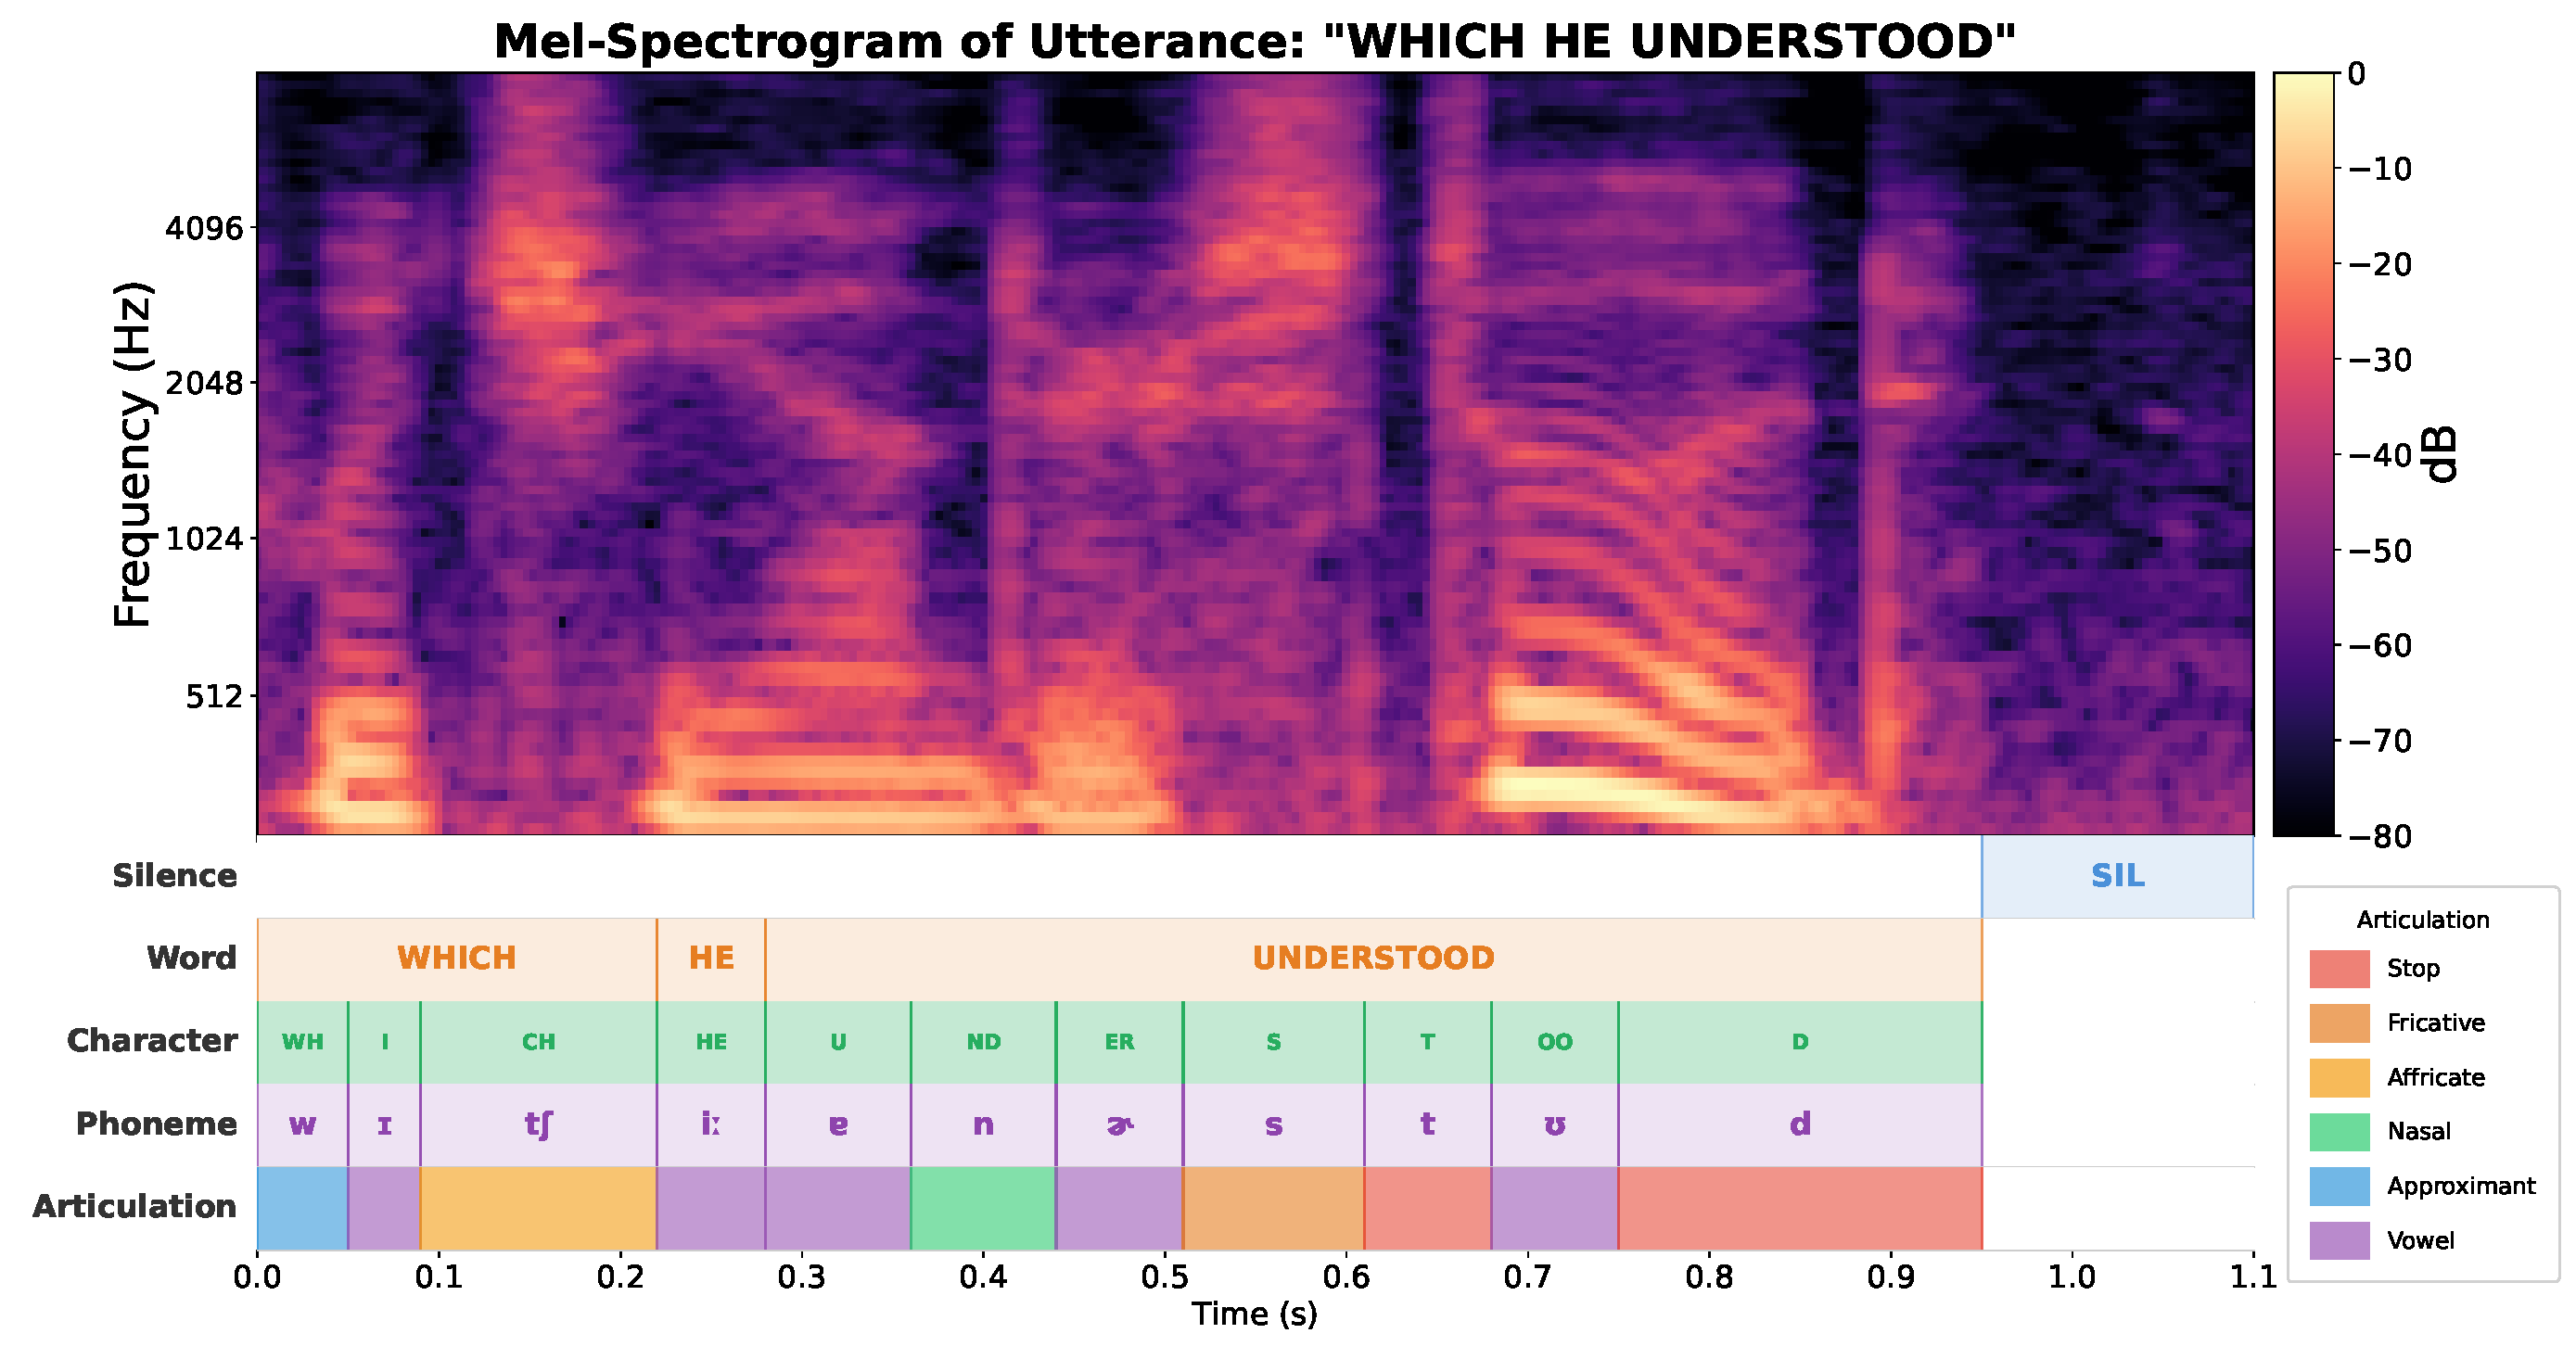
\includegraphics[width=\linewidth]{introduction/images/whichheunderstood_melspec.pdf}
    \caption{A mel-spectrogram of a section of an utterance. Here we see: word, character, phoneme and articulation level alignments. All alignments were generated with the Montreal Forced Aligner (McAuliffe et al 2017). This segment was taken from a LibriSpeech utterance (Panayotov et al. 2015).}
    \label{intro_fig:mel_spectrogram}
\end{figure}

\section{Automatic Speech Recognition}

This volume of information proved difficult for early signal processing to automatically transcribe. However, in 2014 the field of Automatic Speech Recognition (ASR) would change dramatically, with the rise of Deep Neural Networks (DNNs) \cite{hannun2014deep}. DNNs could be trained with labelled data to learn speech features. DNNs start from a random initialisation, so, are not programmed with a priori knowledge of the domain. This allows them to adapt well to the many variations of human speech such as languages, dialects and accents. DNNs were well-suited for learning ASR, wherever sufficient data was available to train them. %DNNs quickly revolutionised fields such as image processing and Natural Language Processing (NLP) \cite{citations_needed}. So when the same techniques were applied to ASR, it quickly outshone all previous approaches.

%This volume of information proved difficult for early signal processing systems to transcribe automatically. The field changed substantially with the rise of deep neural networks (DNNs), which could learn acoustic representations directly from data and reduced reliance on hand-engineered features \cite{hannun2014deep}. DNNs were well suited to automatic speech recognition, provided that sufficient training data was available.

%Early DNN architectures taught Recurrent Neural Networks (RNNs) \cite{Graves2012} to learn sequential labelled speech data using Connectionist Temporal (CTC) Loss \cite{graves2006connectionist}. 

The first DNN architectures learned speech using Connectionist Temporal Classification (CTC) Loss \cite{graves2006connectionist} and learned from thousands of hours of speech. However, CTC required human-transcribed speech data for training, but human transcription is time-consuming and expensive. So, Self-Supervised Learning (SSL) techniques were developed to learn speech without the need for expensive labelling \cite{wav2vec, hsu2021hubert}. They were combined with transformers \cite{vaswani2017attention}, which allow the parallel processing of speech frames, to achieve impressive results. This thesis explores how SSL ASR models learn and how they have been used in modern ASR.

SSL ASR models were able to vastly reduce the cost of training data by bypassing human labelling. It also expanded the number of sources from which data could be extracted. Since SSL loss functions do not have a labelled objective, training must be split into 2 stages: pretraining and fine-tuning. The pretraining stage is done with SSL and then the model is fine-tuned to a labelled objective, such as speech transcriptions, with CTC. To maximise the benefits of SSL, training on large datasets for long periods is done during pretraining. Unlabelled data cannot be utilised in fine-tuning. There are many resources for unlabeled or semi-labelled data, so including them can greatly expand the size of the data pool. The fine-tuning dataset can then be much smaller than the pretraining dataset, since the bulk of learning has already been done.

By making pretrained SSL models open-source\footnote{\hyperlink{https://huggingface.co/facebook/wav2vec2-base}{huggingface.co/facebook/wav2vec2-base}}, they could be fine-tuned to a variety of different datasets. With pretraining, a small amount of fine-tuning data could produce accurate results in multiple speech domains. Some domains, such as small languages or dialects, did not have the large datasets required to train an ASR model from scratch. We refer to these domains as being low-resource. For low-resource domains, SSL pretraining provided an adaptable baseline model that could be fine-tuned to achieve impressive results.

However, it was quickly found that the data used in pretraining has an impact on downstream performance. Most SSL models were pretrained on data from a single language, monolingual pretraining. If the model was fine-tuned to the same language or a related language as the pretraining data, the results could be exceptional. We call this matched-language or related-language fine-tuning. However, if the fine-tuning language was not the same as the pretraining language, it would negatively impact performance. We refer to this as mismatched-language fine-tuning.

The solution, therefore, was to make SSL ASR models multilingual \cite{XLSR-53, whisper}. By pretraining on many different languages, these models were able to substantially improve fine-tuning accuracy for low-resource languages. However, the more languages that were added to pretraining, the worse the performance could be for individual languages. When the size of each model is increased, this trade-off can be offset \cite{babu2021xlsr}. However, as the model size increases the compute power required for both the pretraining and fine-tuning stages also increases. This reduces the benefits of pretraining for low-resource languages. 

This is the point in ASR research that we find ourselves as of the writing of this thesis. The contributions to knowledge in this thesis, therefore, aim to expand our understanding of multilingual SSL ASR. We hope that by contributing, we can help to improve ASR for low-resource languages. These contributions are outlined throughout the rest of this chapter.

%In order to contribute knowledge to the field of ASR, we first explore how SSL ASR models learn speech. We first outline everything currently known about SSL ASR learning. Then we perform experiments to further our knowledge and improve the current performance of multilingual SSL ASR models. We finally suggest how these findings can be used going forward. With these aims in mind, we hope that accurate and efficient ASR can be made available to many more languages and many more people in the future.  


%\section{Thesis Statement}

\section{Research Questions}\label{intro_sec:research_questions}
\iffalse
\begin{itemize}
    \item What do SSL models learn from multilingual data?
    \item We know that SSL models learn aspects of each language but do they learn them equally?
    \item How does the balance of languages in pretraining affect language learning?
    \item Do SSL models learn languages independently?
    \item We know that the XLSR-53 quantizer groups features, so some features at least appear to be language-dependent, but are all of them? 
    \item How does SSL learn imbalanced languages? 
    \item Does SSL rely more on high-resource languages and share more features when learning low-resource languages or do low-resource languages simply suffer?
    \item 
    
\end{itemize}
\fi

This thesis seeks to understand how SSL ASR learn the features of multilingual data. This understanding can then be used to improve ASR for languages across the world. To achieve this, we seek to answer the following research questions:%\newline

%\hl{Do I want to change this to be more like Sam's?}

\begin{enumerate}[start=1,label={\bfseries RQ\arabic*:}]%[RQ*]%[start=0,label={\textbf{RQ}*:}]
    \item How does the balance in hours between different languages included in multilingual SSL pretraining data affect language learning?
    %\begin{enumerate}[start=1,label={\bfseries RQ1.\arabic*:}]
        %\item What does an SSL model learn when a language is low-resource in pretraining?
        %\item Does an imbalance between the language have a negative affect on multilingual learning?
        %\item Does the proportion of data for a language in pretraining affect how well that is learned during pretraining?
        %\item When the languages in the pretraining data are not balanced equally, how much does the model learn about each one?
        \item Do multilingual ASR models use information from related languages learned in pretraining, when performing monolingual fine-tuning?
        %\item How do high-resource pretraining languages interact with the learning of low-resource languages during pretraining?
        %\item Are all languages learned equally in multilingual pretraining, and if not 
    %\end{enumerate}
    \item How do multilingual models learn multilingual phonetic features?
    %\begin{enumerate}[start=1,label={\bfseries RQ2.\arabic*:}]
        \item Do multilingual SSL models learn shared phoneme representations, or do they learn language-specific phoneme realisations separately?
        %\item Articulations are learned to different degrees in English pretraining, is this consistent in multilingual pretraining? \hl{I have removed this from the conclusion for the momemnt. I could change this refernce unseen languges instead...}
        \item How do the languages in pretraining relate to the downstream accuracy of unseen languages?
        \item How does the balance of languages in pretraining affect how each articulation class is learned across languages?%\newline
        %\item Each articulation is learned to a different degree of accuracy in English monolingual pretraining but does this apply in multilingual pretraining?\newline
        %\item Are there any phonetic features that are better shared across languages than others?
        %\item Are all phonetic features language-specific or does the model share any latent space?
    %\end{enumerate}
\end{enumerate}
%\textbf{RQ1} How does the balance in hours of between languages in SSL pretraining affect language learning?


Chapter~\ref{chapter4} primarily addresses \textbf{RQ1} and \textbf{RQ2}. In this chapter, we explore the language-specific subnetworks in the multilingual SSL ASR model XLS-R. We look at which of these language-specific subnetworks are used when fine-tuning. We identify which subnetworks have the lowest Character Error Rates (CERs) across languages. We also isolate languages that are low-resource in pretraining or absent altogether. We then test which language-specific subnetwork produces the lowest CER for these languages. By identifying how subnetworks interact with different languages, we address these research questions. 

Chapter~\ref{chapter5} continues the investigation of language balance in multilingual pretraining, further exploring \textbf{RQ2}. In this chapter, we pretrain 7 multilingual SSL ASR models with different ratios of English and Spanish data. We explore how the ratio between pretraining languages affects fine-tuned error rates. We then probe the models and measure phoneme accuracy and address \textbf{RQ4}. We examine how language-specific realisations of the same phonemes are recognised in each model, answering \textbf{RQ4}. We extend this analysis to measuring the accuracy of phonemes realised in languages unseen in pretraining, which addresses \textbf{RQ5}. We then group phonemes by their Manner of Articulation (MoA) classes and explore how articulations are learned during multilingual pretraining. These findings allow us to answer \textbf{RQ6}.

\newpage
\section{Thesis Outline}
This section gives a high-level outline for each chapter included in this thesis. 

\subsubsection{Chapter~\ref{Chapter2_LR}: Literature Review}
Chapter~\ref{Chapter2_LR} gives a detailed description of the literature that underpins the research throughout this thesis. Section~\ref{lr_sec:asr_early_dnns} covers early uses of DNNs on ASR. We explain the transformer architecture and how processing sequences in parallel changed ASR. Section~\ref{lr_sec:wav2vec2} explains the wav2vec 2.0 SSL ASR model \cite{wav2vec}. We describe the contrastive loss function, the quantizer and how wav2vec 2.0 learns. Section~\ref{lr_sec:multilingual_ssl} details multilingual SSL ASR. We examine the relationship between ASR performance and model size when pretraining on multilingual and monolingual datasets. In Section~\ref{lr_sec:model_compression}, we describe common model compression techniques and go into depth on weight pruning. We explore how language-specific subnetworks can be found within large multilingual ASR models. Section~\ref{lr_sec:model_analysis} details the approaches researchers have taken to analysing SSL ASR models. We cover statistical layer analysis as well as layer analysis through probing. We then review all studies on phoneme and articulation information learned by SSL ASR models. Finally, Section~\ref{lr_sec:datasets_models} presents the models, datasets and training regimes used in the experiments throughout this thesis.

\subsubsection{Chapter~\ref{chapter4}: Language Bias in Self-Supervised Learning for Automatic Speech Recognition}
Chapter~\ref{chapter4} analyses the weight distribution of the multilingual SSL ASR model XLS-R \cite{babu2021xlsr}. Section~\ref{pru_sec:introduction} and section~\ref{pru_sec:background} outline recent advances in multilingual SSL ASR. They cover the size of XLS-R and how model compression techniques aim to reduce the size. They cover how weight pruning can uncover language-specific subnetworks. Section~\ref{pru_sec:experimental_design} outlines our experimental procedure. We describe the architecture of XLS-R and the data it was pretrained on. We detail our pruning strategy and our method for identifying language-specific subnetworks. In Section~\ref{pru_sec:experimental_results}, we identify multiple language-specific subnetworks within XLS-R. We then test the fine-tuned CER on matched-languages and mismatched-languages. We analyse their weight distributions and where language-specific subnetworks overlap. Then, in section~\ref{pru_sec:discussion} and Section~\ref{pru_sec:conclusion} we discuss our findings. 

\newpage
\subsubsection{Chapter~\ref{chapter5}: Data Balance and Learning in Multilingual SSL}
In Chapter~\ref{chapter5}, we measure how the ratio between the number of hours in each pretraining language relates to the downstream performance of multilingual SSL ASR models. Section~\ref{ed_sec:introduction} and section~\ref{ed_sec:background} outline the trade-off between multilingual and monolingual SSL pretraining. This section also covers methods used to analyse how SSL ASR models learn speech, including statistical layer analysis and layer probing. In section~\ref{ed_sec:experimental_design}, we outline our experimental methodology. We describe each of our pretraining, fine-tuning and layer probing strategies. We then outline how we will use these strategies to understand how SSL learns multilingual phonetic features. In section~\ref{ed_sec:experimental_results}, we present our results. We show how the ratio between pretraining languages relates directly to fine-tuned error rates. We then prove that individual phonemes are learned as language-specific realisations. We finally present phoneme accuracy at an articulation level. WWe find that MoA classes are not learned equally across languages and several factors can contribute to high MoA class accuracy. Finally, in section~\ref{ed_sec:discussion} and section~\ref{ed_sec:conclusion} we discuss our findings. 


\subsubsection{Chapter \ref{Chapter6}: Conclusion}
In Chapter~\ref{Chapter6} we outline the findings and contributions raised in this thesis. In section~\ref{conc_sec:summary} we summarise Chapter~\ref{chapter4} and Chapter~\ref{chapter5} and whether this thesis answers the research questions. In section~\ref{conc_sec:limitations} we outline some limitations to the experiments in this thesis. We reflect on how those limitations affect our interpretation of the findings in this thesis. In section~\ref{conc_sec:future_work}, we outline the future work that could be done based on the contributions of this thesis. Finally, in section~\ref{conc_sec:final_remark} we outline the final remarks on this thesis.

%\section{Contributions}
\section{Research Contributions}
\iffalse
\begin{itemize}
    \item Chapter 4
    \item Contributions to Language-specific subnetworks
    \item identifying that 80\% of the subnetworks overlap
    \item Identifying that new languages learn from English weights
    \item Identifying that XLS-R can be reduced in size by up to 60\% with no impact on WER and 70\% with little impact
\end{itemize}

\begin{itemize}    
    \item Chapter 5
    \item Identifying exactly how much multilingual data affects finetuned WER
    \item How well phonemes that exist in pretraining are recognised by the model
    \item How well phonemes that don't exist in pretraining are recognised
    \item How language affects phonemes, does a phoneme that exists in both languages get high accuracy or has the model learned realisations separately?
    \item How different MoA are understood by multilingual SSL models
    \item How the number of interval counts in pretraining relates to MoA class accuracy
    \item How phoneme interval counts in pretraining and probe training relate to accuracy
    \item How interval counts in a class relate to unseen phoneme accuracy.
\end{itemize}
\fi

%Here we summarise the contributions to knowledge as follows:

\subsubsection{Contributions relating to Chapter~\ref{chapter4}.}\label{intro_subsec:contributions}

The contributions outlined in this chapter were presented at the IEEE, Spoken Language Technology (SLT) conference, in Macau in 2024. 

\begin{enumerate}
    \item \textbf{Sparsity in Multilingual XLS-R}

    We compare the sparsity that different language-specific subnetworks can be pruned to without increasing the error. We show in Chapter~\ref{chapter4} that, for all languages, XLS-R can be pruned to 50\% sparsity without any increase in the error rate. We further show that, for all languages, XLS-R can be pruned to 70\% without a significant increase in error.

    \item \textbf{Subnetwork Performance}
    
    Previous studies had shown that fine-tuning to matched-language subnetworks produced the lowest CER. However, for XLS-R, this is not true. The best performing subnetwork comes from English. English is the language that contributes the most hours to the pretraining data. We compare the CER produced by each language-specific subnetwork, at >=70\% sparsity, when fine-tuned to multiple languages. We find that the English language-specific subnetwork produces the lowest CER for all languages. This is true even when compared to matched-language fine-tuning for other languages. 

    %\item \textbf{Subnetwork Adaptability}

    %We show that pruning with the English language-specific subnetwork can lower CER even after fine-tuning XLS-R to a language other than English. We fine-tune XLS-R to Spanish and prune with the English subnetwork. We show that this pruned model produces lower CER for English, Asturian and Xhosa, when compared to pruning the same model to the Spanish subnetwork. The matched-language, Spanish, is the only language that increases in CER.


    %With this finding we test the performance of fine-tuned subnetworks on related and unrelated languages. We fine-tune Spanish and English subnetworks on 4 languages: English, Spanish, Asturian and Xhosa.  Spanish, Catalan and Asturian are all closely related Romance languages originating in Spain. and the CER\thoughts{Need to define CER/WER earlier} 

    \item \textbf{The Overlap Between language-specific subnetworks}

    We test the Intersection Over Union (IOU) between language-specific subnetworks. The IOU measures how many weights each subnetworks share. Previous studies showed language-specific subnetworks to have a >90\% IOU for models trained from scratch. For XLS-R, we show the IOU is always between 80\% and 90\%. We further show that the English subnetwork had the highest IOU with the pretrained model, before fine-tuning. Previous studies had not measured how language-specific subnetworks generated from related languages interact. So, finally, we show that Asturian and Catalan subnetworks have a higher IOU with the English subnetwork than the Spanish subnetwork.
    
\end{enumerate}

\subsubsection{Contributions relating to Chapter~\ref{chapter5}.} 

Prior studies have shown that wav2vec 2.0 learns phonemes and manner of articulation during pretraining. The contributions in this chapter explore how multilingual pretraining affects phonetic feature learning. The contributions in this chapter have yet to be published.

\begin{enumerate}
    \item \textbf{How language balance in pretraining reflects Error Rate}

    Previous studies show that monolignual matched-language pretraining and multilingual related language pretraining can decrease fine-tuned CER. Multilingual mismatched pretraining can increase CER when compared. We prove that the ratio of matched to mismatched languages also relates directly to fine-tuned CER. As matched-language data is increased in pretraining, fine-tuned error reduces proportionally. Inversely, as the amount of mismatched data is increased, the CER increases proportionally. We further prove that this relationship is also true for related languages. As related language data in pretraining increases, fine-tuned CER reduces proportionally.

    \newpage
    \item \textbf{Phonemes are learned as language-specific realisations}

    We find that language-specific phoneme realisations are learned separately in pretraining. As matched-language data is increased in pretraining, matched-language phoneme accuracy increases proportionally. As the mismatched-language increases, mismatched-language phoneme accuracy decreases proportionally. We also test unseen languages, those that are not included in pretraining. Unseen related language phonemes that exist in pretraining have a higher average accuracy than phonemes that do not exist in pretraining. This is true for unseen mismatched language phonemes as well.

    %\item \textbf{How language balance in pretraining reflects Phoneme Accuracy}

    \item \textbf{How multilingual pretraining learns articulation}

    previous studies have shown that SSL ASR learn articulations, however multilingual articulations have not been explored. We find that multilingual SSL ASR does not learn MoA classes equally. Multiple factors can contribute to how well multilingual SSL has learned an articulation class. For each class the dominant factor can be different. These factors include: pretraining class exposure, the ratio between pretraining languages and the language a phoneme is spoken in. 
    
    %In some cases a MoA class with high exposure in pretraining can have high average accuracy. In other cases one of the pretraining languages can produce higher accuracy for a class than the other. This can be true even for phonemes spoken in unseen languages. The ratio between the pretraining language hours can then further impact this class accuracy. We present these and other findings on multilingual MoA accuracy.
    
    %For example, vowels are high-resource across all language ratios in pretraining. Vowels also have a high average accuracy across all languages. Fricatives that do not appear in either pretraining language have higher accuracy when compared to other MoA classes. Spanish trills in pretraining do not increase Polish trill accuracy. We present these and other findings on multilingual MoA accuracy.

\end{enumerate}

\section{Publications}

%\textbf{Storey, E.}, Harte, N., Bell, P. (2024).

\begin{enumerate}
    \item \textbf{Storey, E.}, Harte, N., and Bell, P. (2024) "Language Bias in Self-Supervised Learning For Automatic Speech Recognition," \textit{IEEE Spoken Language Technology Workshop (SLT)}, Macao, 2024, pp. 37-42, doi:10.1109/SLT61566.2024.10832268.
\end{enumerate}

\nomenclature[A]{CTC}{Connectionist Temporal Classification}
\nomenclature[A]{ASR}{Automatic Speech Recognition}
\nomenclature[A]{DNN}{Deep Neural Network}
\nomenclature[A]{SSL}{Self-Supervised Learning}

%\input{background/background.tex}
%\input{project/project.tex}
\input{2_chapter2/chapter2.tex}
%\input{3_chapter_3/chapter_3_new}
\input{4_chapter_4/chapter4.tex}
\input{5_chapter5/chapter5}
%\input{6_discussion/discussion.tex}
\chapter{Conclusion}\label{Chapter6}
\iffalse
\begin{itemize}
    \item Mark conclusion: 7 pages, no discussion section
    \begin{itemize}
        \item Conclusions/Summary: 4 pages
        \item Future Work: 2.5 pages
        \item final remarks: 0.5 pages
        \item blank page: 1 page
    \end{itemize}
    \item George conclusion: 12 pages, no discussion section
    \begin{itemize}
        \item Summary + Significance: 3 pages
        \item Context: 0.5 pages
        \item limitations: 0.5 pages
        \item "What went wrong": 1 page
        \item Broader Impact: 0.5 pages
        \item Future Work: 5.5 pages
        \item Final remarks: 0.5 pages
        \item blank: 0.5 pages
    \end{itemize}
    \item Rishabh: 5 pages, no discussion
    \begin{itemize}
        \item Summary/Contributions: 2 pages
        \item Discussion: 0.5 pages
        \item future work: 2 pages
        \item blank: 0.5 pages
    \end{itemize}
    \item Sam: 8 pages, no discussion
    \begin{itemize}
        \item Summary/ Contributions: 4 pages
        \item Related work: 1.5 pages
        \item Future Work: 2.5 pages
        \item Concluding remoarks: 0.5 pages
    \end{itemize}
    \item Ayushi: 5 pages, no discussion
    \begin{itemize}
        \item Summary: 2 pages
        \item Context: 0.5 pages
        \item Limitations: 0.5 pages
        \item future work: 2 pages
        \item Final remark: 0.5 pages
        \item blank: 0.9 pages
    \end{itemize}
\end{itemize}
\begin{itemize}
    \item My Conclusion:
    \item Summary/Conclusion
    \item Limitations
    \begin{itemize}
        \item Do I want a george style "what went wrong"?
    \end{itemize}
    \item Future Work
    \item Final Remarks
\end{itemize}
\fi

\iffalse
\hl{Brief Intro paragraph} 2-paragaphs
\begin{itemize}
    \item restate overall aims and problems
    \item \hl{I don't necessarily need this, skip for now}
\end{itemize}
\fi


\section{Summary}\label{conc_sec:summary}
\iffalse
\hl{2-4 pages}
\begin{itemize}
    \item \hl{I should relate to research questions here}
    \item Chapter 3 and model pruning
    \item what was achieved and what we reasoned
    \item Chapter 4 and model probing
    \item what was achieved and what we reasoned
    \item Context/Limitations section
    
\end{itemize}

\hl{Overall summary of the field and our aims}
\begin{itemize}
    \item We can talk a little here about the concept of pretraining introduce the idea of the resources it takes to pretrain a big model
    \item How we as downstream researchers, do not have the resources to train them ourselves
    \item how multilingual pretraining is not deeply thought through, and a see what sticks approach is very common
    \item This thesis is all about picking that apart and finding out how they work and if we can improve upon that
    \item 
\end{itemize}
\fi

In this chapter we will summarise the major findings across this thesis and how they align with our research questions from section~\ref{intro_sec:research_questions}.

\subsection{Language Bias in Self-Supervised Learning}

In Chapter~\ref{chapter4}, we dissect the multilingual SSL ASR model XLS-R \cite{babu2021xlsr} by using LTH \cite{frankle2018LTH} to identify language-specific subnetworks. First, we find the highest sparsity that XLS-R can be pruned to without increasing CER. We find that with unstructured pruning, the model can be pruned to 50\% without any increase in CER and to 70\% with only a marginal increase. This finding is consistent across all languages tested fine-tuning to monolingual subsets of the FLEURs \cite{FLEURS} multilingual dataset.

For sparsities >=70\%, we then fine-tune each of these subnetworks to a matched, related or mismated language and measure CER. This approach is our first step to answering \textbf{RQ1}, which asks how the balance of languages in pretraining affects downstream learning. Previous studies had identified language-specific subnetworks and fine-tuned them with a matched-language. This approach had been shown to produce highly sparse, low-error networks \cite{PARP, Lu_Language_adap_xlsr, yang2023learning}. However, little work had been done to analyse the weight distributions of these subnetworks. %For instance, whether a language-specific subnetworks could be adapted to related or mismatched languages. Whether subnetworks drawn from high-resource languages in pretraining would produce more beneficial weights. How language-specific subnetworks interact with one another, and whether there are linguistic relationships behind them. 

For \textbf{RQ1}, we start by comparing the fine-tuned CER of multiple language-specific subnetworks. We found that across all languages, at >=70\% sparsity, the English language-specific subnetwork produced the lowest CER. This was true even when compared to subnetworks of related languages. English is also the language with the most hours in pretraining, which shows that language balance has a substantial impact on subnetwork performance. Fine-tuning the English subnetwork to Asturian even resulted in lower CER than fine-tuning the Spanish subnetwork to Asturian. This leads us to address \textbf{RQ2}, which asks whether, during fine-tuning, multilingual models use information learned in pretraining from related languages. Through our fine-tuning of the language-specific subnetworks, we have shown that XLS-R is not using weights learned from related languages. 

To further investigate \textbf{RQ2}, we assess the IOU between language-specific subnetworks. We find that the English subnetwork has the most overlap with the pretrained XLS-R before it is fine-tuned. Therefore, the weight distribution of XLS-R changes the least when fine-tuning to English compared to other languages. We further test language relationships by comparing the English subnetwork to languages originating in Spain. We find that the English language-specific subnetwork had a high IOU with both Catalan and Asturian. We then measure the IOU between the Spanish subnetwork and subnetworks for Catalan and Asturian. The IOU between the Spanish regional languages was lower than the IOU found between them and English. This further shows that when fine-tuning, XLS-R relies on weights learned from English. It is not, therefore, using information learned from related-languages. 

%By analysing the behaviour of and the relationship between language-specific subnetworks, we provide the first steps in understanding the behaviour of multilingual SSL ASR models. The findings of Chapter~\ref{chapter4} suggest that the distribution of languages in pretraining has an impact on downstream performance. This impact has been trained into the model during the pretraining stage. In order to answer \textbf{RQ1}, we must next understand how multilingual SSL ASR models learn speech.

\subsection{Data Balance and Learning in Multilingual SSL}
%In Chapter~\ref{chapter4} investigated how the balance of languages in XLS-R pretraining affected downstream CER. However, we did not compare our findings to a multilingual model with a different balance of languages. Without this comparison, we have not yet answered the question on language balance from \textbf{RQ1}.

In Chapter~\ref{chapter5}, we continue investigating \textbf{RQ1} by pretraining 7 separate base wav2vec 2.0 models with different balances of 2 pretraining languages. We pretrain 2 monolingual models, 1 pretrained on English \cite{librispeech} and 1 on Spanish \cite{MLS}. We then train 5 more models with different ratios of Eng/Spa data: 800/100, 600/300, 450/450, 300/600. 100/800. We first fine-tune these models to English and Spanish data. We find that for both languages, downstream CER decreases proportionally to the amount of matched-language data in pretraining. We then fine-tune to multiple FLEURs \cite{FLEURS} languages. We find that this proportional increase in accuracy is true for related languages in pretraining as well. For unrelated language, there is no clear correlation between pretraining language balance and downstream CER. %These findings show that the balance of hours between multiple languages in pretraining directly relates to the model's multilingual performance.

%These findings validate our previous answers to \textbf{RQ1} and \textbf{RQ2} based on the findings of Chapter~\ref{chapter4}. 

%To understand how the balance of languages has this effect, we must next understand how multilingual SSL ASR models learn speech during pretraining. Previous studies have shown that English monolingual SSL ASR models learn phonetic features during pretraining \cite{pasad2021layer, english2022domain, wells2022phonetic}. Without any fine-tuning, these models are able to perform phoneme recognition with high accuracy. 

Our next experiments then address \textbf{RQ3}, which asks how multilingual SSL ASR models learn phonetic features. We first test our pretrained models for phoneme accuracy through MLP probing. We first collect phoneme intervals with the MFA \cite{mcauliffe2017montreal} from English, Spanish, French and Polish data, \cite{librispeech, MLS}. We then train probes from the layer 7 outputs of each model and collect phoneme accuracy from our test data.

To answer \textbf{RQ3}, we first ask whether SSL ASR models learn multilingual phonemes as shared or separate realisations, which forms \textbf{RQ4}. We group phonemes by the pretraining language in which they appear. We found that phonemes shared across the English and Spanish phoneme inventories have a higher average accuracy than phonemes unique to either language. We also find that both English and Spanish phonemes increase in accuracy proportionally to the amount of matched-language data in pretraining. These experiments revealed that phonemes are learned as separate realisations. 

In this section, we also address, which asks how languages unseen in pretraining interact with phoneme representation. Our experiments show that French and Polish phonemes have higher accuracy when they appear in the pretraining language inventories. Phonemes that are unique to each language have low accuracy by comparison. Therefore, unseen languages benefit from phoneme representation in pretraining, even from mismatched languages.

%So, we also found that having a phoneme represented in pretraining still benefits phoneme accuracy for unseen languages.\thoughts{I could change RQ5 to be about unseen and add it here}

%To understand why unseen languages still benefit from phoneme representation in pretraining, we can first break down phonemes into their MoA classes. It has been shown that the pretrained monolingual English wav2vec 2.0 can identify articulations \cite{english2022domain}. However, it does not learn each MoA class to an equal accuracy. In pretraining, both wav2vec 2.0 and XLS-R assign more codebook entries to certain MoA classes, such as vowels, compared to others \cite{quantizer_entries_paper}, when tested on English phonemes \cite{timit}. 



%This leads us to \textbf{RQ6}\thoughts{expand on RQ6}\thoughts{I have skipped RQ5 for now, it overlaps with the other RQs so I don't think I need it. OR I need to change it, to something about how multilingual quantizers learn.} which asks how the balance of languages affects the learning of articulations.\thoughts{Can probably move this later.} .\thoughts{probably need to define the test languages them somewhere} 

To further understand these findings, we address \textbf{RQ6}, which asks how multilingual language balance affects MoA learning. We plot the average MoA class accuracy on each model for each of our 4 test languages searately. We first see that high-resource matched-language models always produce the highest MoA class accuracy. However, the extent to which matched-language pretraining is beneficial to phoneme accuracy differs by class. Spanish vowels, for example, have high accuracy across all 7 models, which is not true of English. Vowels that exist in both Spanish and an unseen language also have high accuracy. Vowels that exist in English and an unseen language have low accuracy by comparison. However, direct phoneme or MoA class representation in pretraining is not always enough to increase accuracy for unseen languages. Polish trills, for example, have low accuracy even on the Spanish monolingual model.

To control for low-resource phonemes in tests we next weight MoA phoneme accuracy by their number of intervals. For nasals and fricatives, we find that the average accuracy for all languages increases. For certain languages, the increase in accuracy is large and this is not the case for other MoA classes. We then plot phoneme accuracy against probe test interval counts with scatter plots. The number of intervals in the probe testing data is shown to correlate with high phoneme accuracy. We also plot accuracy against pretraining interval counts and find that the number of intervals in pretraining can also correlate with phoneme accuracy. Low-resource Nasals and fricatives are often found to have high accuracy regardless of interval counts in pretraining. These classes can be low accuracy for very low-resource phonemes, where there are less than 500 intervals in test. However, for low-resource, more than 500 intervals, nasals and fricatives often have high accuracy, compared to low-resource phonemes in other classes. This suggests that, above a certain threshold of test intervals, MoA class alone can be a correlating factor to high accuracy.

%%%%%%%%%%%%%%%%%% MAYBE I CAN USE THIS FOR THE FINAL THOUGHTS  %%%%%%%%%%%%%%%%%%%%%

%Across these findings we see that the answer to \textbf{RQ6} is multi-faceted. Matched-language pretraining exposure consistently benefits MoA class accuracy. To a lesser extent, mismatched pretraining exposure can also benefit MoA class accuracy. Language selection is also important to high MoA accuracy. In certain cases the class itself is simply well learned by wav2vec 2.0.

%Overall, we answer \textbf{RQ1} by stating that this thesis proves the balance between languages in pretraining does directly relate to language learning. The more matched-language data there is in SSL ASR pretraining, the higher the matched and related language downstream accuracy becomes. For unseen languages, balance is less important, as long as a model has been trained on phonemes that exist in the unseen language. Articulation plays a factor, but the factors can be MoA class or language specific.


\section{Limitations}\label{conc_sec:limitations}

\subsubsection{Probing Data}
There are a number of limitations to the findings outlined in section~\ref{conc_sec:summary} that must be addressed. When probing wav2vec 2.0 models, \iffalse we test the average accuracy of each individual phoneme. We then compare this to the average phoneme accuracy weighted by the number of phoneme intervals in the test data. The latter of these approaches highlights that phonemes with more examples in test have averagely higher accuracy. The scatter plots confirm that the number of phoneme intervals in the test dat,a correlates with high individual phoneme accuracy.\fi we plot MoA weighted accuracy and scatter plots. These plots show that the number of phoneme intervals in the probe testing data correlates with phoneme accuracy. Therefore, the first limitation to note is that the MLP probes themselves add bias towards high-resource phonemes. 

Phonemes that are low-resource in test may lower the average accuracy of a phoneme. These low-resource phonemes are usually low-resource in the probe training data as well. It could therefore be that the probes have not learned the representations for these phonemes well. We see in appendix~\ref{app_sec:chapter_5_appendix}, table~\ref{app_tab:phoneme_counts_per_language_vaid_1} that some phonemes have less than 10 intervals in the test data. It is possible that these phonemes have been misaligned. This is a limitation of using forced alignment rather than annotated phonemes. 

By increasing the number of hours of test and training data, these issues could be mitigated. Early in the research process, we ran a test that trained our probes on 100 hours of LibriSpeech data instead of 10 hours \cite{librispeech}. We found that the average phoneme accuracy did increase when training on 100 hours of data. However, the increase was small relative to the increase in training time. We decided, therefore, that we would not train on the larger dataset. By training the probes on the smaller dataset, we may have impacted the final results. However, very low-resource phonemes, with less than 500 intervals, are still rare in both the test and training data. Therefore, we do not believe that the 100 hour datasets would have substantially changed the overall findings.

\subsubsection{Available Compute Power}

Compute power was a common limitation, often constraining the scope of potential experiments. However, this constraint also inspired the research direction of this thesis. Before performing pruning experiments on XLS-R we focussed on training low-parameter CNN models with approximately 6M parameters. We trained Quartznet15x5 \cite{quartznet} on LibriSpeech \cite{librispeech} and MLS languages \cite{MLS} as well as accented English data \cite{aesrc2020}. However, the results produced a high WER compared to SOTA models at the time. So we attempted strategies such as data augmentation, layer freezing and varying the learning rate scheduler \cite{some citations here}. However, we could not find an approach that competed with SSL transformer models. This line of research was eventually dropped. 

The experiments in Chapter~\ref{chapter4} were performed at The University of Edinburgh, where we had access to a larger cluster of GPUs. This extra compute power allowed us to focus on the large SSL ASR model XLS-R \cite{babu2021xlsr}. We were able to study exactly what made it perform better than our smaller models. However, even here, we did not have the resources to train the larger 2B parameter XLS-R version. This limitation inspired the use of model compression techniques seen in this thesis. Through LTH \cite{frankle2018LTH}, we showed, among other findings, how much this model could be reduced in size without affecting performance.  

The next direction was originally to experiment with knowledge distillation \cite{distillation}. The work had moved back to Trinity College Dublin and we now had access to more compute. However, again, the results were uninspiring when compared to other methods. Optimisation was difficult due to the large amount of GPU memory used in model distillation. This limited the directions we could expand these experiments into, despite our increased compute power. We shifted the scope of the experiments instead to pretraining multiple base wav2vec 2.0 models, something we now had the resources to do. This allowed us to emulate some of the behaviour of XLS-R and analyse language balance in multilingual SSL. This eventually formed the contributions presented in Chapter~\ref{chapter5}

When we were training Quartznet15x5 \cite{quartznet} Meta\thoughts{technically Facbook research back then} had recently published wav2vec 2.0. Quartznet15x5 had 6M parameters and wav2vec 2.0 large had 317M. When we had access to increased compute resource, we would experiment with the 0.3B version of XLS-R and later pretrain the 0.1B wav2vec 2.0 model. During the same period we conducted these experiments, Meta would publish LLaMA \cite{llama_citation}. LLaMA is a 65B parameter Large Language Model (LLM). Google would then create their own LLM, Gemini, which is estimated to have a parameter count of 1.5T \cite{howtoreference?}. Although Gemini's parameter count has not, to this point, been officially disclosed by Google. 
%We have never been able to compete with the computation required to train these models.\thoughts{reword} As well, many researchers in low-resource fields have even fewer resources than we did. 

This disparity in resources between companies and research institutions highlights the need to understand how SSL models learn. With a better understanding, we can optimise these models to achieve better results with less computational resources. We hope, therefore, that this particular limitation has translated into a contribution that helps those with few resources of their own.


\section{Future Work}\label{conc_sec:future_work}

In this section, we will outline some avenues for future work based on the points raised in section~\ref{conc_sec:summary} and section~\ref{conc_sec:limitations}.

\subsection{Model Compression}

A natural direction to take the results in Chapter~\ref{chapter4} is to further experiment with model compression. First, our findings could be applied to model distillation \cite{distillation}. Distillation has been successful in producing high-accuracy compressed models \cite{chang2022distilhubert, sanh2019distilbert}. A future project could compare the results of distilled XLS-R models when training the student model with different languages. 

Future work could also apply our findings in Chapter~\ref{chapter4} to structured pruning.  Structured pruning removes entire nodes in a network. Compressed networks can be deployed with structured pruning, without the need for specialist hardware or software. This is not the case for the unstructured pruning used in Chapter~\ref{chapter4}. Future work could test if the English language-specific subnetwork still performs well with structured pruning.

Finally, we would like to see more work analysing language-specific subnetworks using unstructured pruning. We showed that at 70\% sparsity CER did not substantially increase. The English subnetwork was able to produce low CER for all languages. Additionally, 80\% or more of the weights between language-specific subnetworks overlap. It is important, therefore, that we identify the information encoded in this small portion of remaining weights. 

%Pasad et al. \cite{pasad2021layer} identified that weights in layers containing acoustic information change less after fine-tuning than deep layers containing semantic information. Fine-tuning is required before applying LTH \cite{frankle2018LTH} to identify a language-specific subnetwork. So, analysing whether these impactful weights are acoustic or semantically driven is important. Global pruning was used in our research so further analysis could be done to analyse the sparsity at each layer. This may give insight into whether English acoustic or semantic data is encoded in the approximately 20\% of weights that do not overlap. 

\iffalse
\hl{2-3 pages depending on whether I write it up}
\begin{itemize}
    %\item Analysis work and short term experiments %\hl{There has to be a better phrase for this}
    \iffalse
    \item Generate and analyse scatter plots with phoneme accuracy vs  pretraining interval count
    \begin{itemize}
        \item We expect high accuracy to correlate with high pretraining count
        \item We expect low accuracy to correlate with low pretraining count
        \item we expect this relationship to be linear
        \item However, the unseen languages have many phonemes that are not in pretraining
        \item We test the test data interval counts as well
    \end{itemize}
    \item Generate and analyse scatter plots with phoneme accuracy vs  test data interval count
    \begin{itemize}
        \item We expect high accuracy to correlate with high test count
        \item We expect low accuracy to correlate with low test count
        \item However, we expect this to be more noisey, with certain phonemes not matching the patterns i.e. polish trills
    \end{itemize}
    
    \item Fit a linear regression model to several variables: pretraining interval count, test interval count, phoneme accuracy, language, MoA class, matched-language condition.
    \begin{itemize}
        \item This allows a more complex analysis of all of the relationships explored in this chapter
        \item Linear regression allows us to see which factor is most relevant to high dowsntream accuracy.
        \item We could also add other broader factors, such as phoneme time length to the list of factors.
    \end{itemize}
    \fi
    \item \textbf{Short-term experiments}:
    \item This experiment would be a short time commitment.
    \item No one has done a clear study on how the wav2vec 2.0 quantiser learns multilingual phonemes.
    \begin{itemize}
        %\item \hl{ADD SOMETHING HERE ABOUT ANALYSIS OF THE CODEBOOK}
        \item With the English monolingual model from the wav2vec 2.0 paper, each English phoneme was shown to have a responding codebook entry \cite{wav2vec}.
        \item The XLSR-53 paper claims that the contrastive loss function for wav2vec 2.0 makes the quantiser share the same speech representations across languages \cite{XLSR-53}.
        \item However, they never actually prove that it did learn them together by repeating the same experiment on the codebooks from the wav2vec 2.0 appendix.%, we could do this easily by seeing if the same phoneme in English and Spanish use the same entry or if the quantiser assigns them separate entries.
        \item I could also look at whether certain MoA classes are more represented in the codebook, similar to this study on vowels \cite{cambara2022recycle}.
        \item This is a big open goal in the literature, and our models are well set up for that analysis. It would also be a relatively quick experiment to run.
        %\item XLS-R paper does cover this lightly as well and states that it does skew towards English
        \item Some relevent references: \cite{wang2025normalization, linke2023self, lee2024balanced}
    \end{itemize}
    \item \textbf{Long term experiments}: %\hl{AGAIN, NEEDS BETTER WORDING}
    \item Both of these experiments would be a big time commitment.
    \item \textbf{Experiment 1}: We continue on from the short-term experiment, if multilingual wav2vec 2.0 models are found to be separating the same phonemes into different codebook entries when spoken in different languages.
    \begin{itemize}
        \item A new model with the same pretraining data mixes could be pretrained with one or all of the following strategies:
        \item \textbf{Strategy 1}: The XLSR multilingual pretraining strategy for encouraging low-resource languages could be tweaked.
        \item \textbf{Strategy 2}: The $\tau$ variable in the loss function that increases diversity of entry use could also be tweaked.
        \item Building a variable into the loss function that encourages or forces wav2vec 2.0 to use the same entry for a single phoneme, even when spoken in different languages, could improve multilingual learning. 
        \item If this could be achieved, many more entries could be freed up to learn more fine details about each language.
        \item \textbf{Strategy 3}: Just massively increasing the number of codebooks. If the quantiser learns multilingual phonemes in separate entries, then increase the number of entries so it has more space to learn all of the information.
        \item Option 3 would increase the number of learnable parameters in the model, but by a much smaller amount than increasing the encoder size, as done for XLS-R. This might be an acceptable trade-off to improve multilingual accuracy.
    \end{itemize}
    \item \textbf{Experiment 2}:  Given the findings of the interval counts experiments, we would try to construct a dataset that would be optimal for pretraining on an unseen language.
    \item \textbf{Option 1}: A dataset where each MoA class is balanced in the number of interval counts and no single phoneme is very low-resource. This would create a very generalisable pretraining dataset. It probably wouldn't achieve very low error rates, compared to high-resource monolingual pretraining. However, it could be very adaptable for unseen, low-resource languages.
    \item \textbf{Option 2}: We construct a pretraining dataset that has the same phoneme inventory and interval counts as a single unseen language. The aim of this dataset is to produce an SSL model that could rival monolingual or related language pretraining, without including any matched-language data. This would show exactly how effective phoneme exposure in pretraining is to downstream accuracy.
    %\begin{itemize}
     %   \item This scenario is produced if pretraining interval count is clearly has the most correlation to downstream accuracy.
    %\end{itemize}
\end{itemize}
\fi

\subsection{Linear Regression for Phoneme Accuracy}

To continue our analysis of phoneme accuracy in Chapter~\ref{chapter5}, we could apply linear regression to our phoneme accuracy data. Linear regression models the relationship between a set of weighted variables and a continuous output. It is trained to minimise prediction error by learning which weights correlate to the highest accuracy across all outputs in the data. Some initial models were run, which showed that the number of phoneme intervals in both probe training data and pretraining data had a high correlation to phoneme accuracy. However, time constraints meant that complex models, including MoA class interval counts or language-specific models, could not be explored. 

\subsection{Quantized Latent Speech Features in Multilingual SSL}

In section~\ref{lr_subsec:analysis_quantizer} we review studies on quantized phonetic features in pretrained wav2vec 2.0. Baevski et al. \cite{wav2vec} identified that wav2vec 2.0 quantizer codebook entries correlates to a specific English phonemes. Later, Conneau et al. \cite{XLSR-53} showed that XLSR-53 codebook entries clustered together by language. Abdullah et al. \cite{abdullah2023information} then showed that XLS-R codebook entropy was only at 24.2\% when testing English phonemes from TIMIT \cite{timit}. The work in Chapter~\ref{chapter5} shows that phonemes are learned as language-specific realisations. Using only English phonemes to test codebook entries could explain the low entropy in XLS-R. The remaining entries that were not activated in their study may be phoneme realisations in other languages.

Continuing from our work in Chapter~\ref{chapter5}, the quantized features in the codebooks for our 7 models could be analysed. We can first test the monolingual models by measuring entropy across all phonemes in only matched languages. This will give us monolingual baselines for codebook entropy. We can then analyse the entropy in our mixed-language models for both matched and mismatched languages. The balanced 450/450 model can tell us how wav2vec 2.0 learns phoneme realisations across the two languages. The 800/100 and 100/800 models will tell us whether language scarcity in pretraining encourages cross-lingual sharing of entries. Finally, we can map language-specific phonemes to codebook entries and compare the results to our entropy findings. With this information, we could redesign the upsampling training strategy in XLSR-52 \cite{XLSR-53} to share more cross-lingual realisations. This could be done by reducing entropy factors in the Loss function, to encourage fewer entries to be used overall. We could also use MFA alignments to decide when entropy should be reduced or increased. 

\subsection{Pretraining Dataset Composition}

We found in Chapter~\ref{chapter5} that phonemes seen in pretraining had the highest average accuracy. This was true when comparing phonemes spoken in both seen and unseen languages. Building on these findings, we could design a synthesised language dataset using multilingual phoneme realisations. This dataset could test how much phoneme pretraining exposure impacts model accuracy.

This synthesised dataset would take utterances from multiple languages to mimic the phonetic structure of one excluded language. The phoneme inventory of the synthesised dataset would be identical to that of the excluded language. The number of intervals per phoneme would also be identical to the excluded language. Given our findings on MoA classes in Chapter~\ref{chapter5}, articulations could also be selected from languages that produced the highest accuracy in each class.

Two SSL models could then be pretrained, one with the synthesised dataset and one with real data from the excluded language. The phoneme accuracy and fine-tuned error from both models could then be compared. We would aim to produce relative performance to a model pretrained on the excluded language without including any of the target language data. 

A comparison could also be made to an open-source multilingual model such as XLSR \cite{XLSR-53, babu2021xlsr}. We would expect the model pretrained on the synthesised dataset to produce better accuracy for the excluded language than the open-source multilingual model. If this were the case, then we could show the benefits of carefully selecting pretraining data. This experiment would also prove that carefully selected data from other languages can be used to augment low-resource datasets.

%A further dataset could be designed for high-performance multilingual pretraining. It would include a broad phoneme inventory and each phoneme in the inventory would be high-resource, with many intervals in pretraining. A model pretrained on this dataset could then be compared to the multilingual SOTA. %Pretraining with this dataset would aim to produce a high-accuracy multilingual model. If the pretraining dataset is effective, the size of the model could be reduced to the smallest possible size. We would aim to achieve lower error with fewer parameters than the multilingual SOTA.


%\section{Contributions}\label{conc_sec:contributions}
%\hl{0.5-1 page}
%\begin{itemize}
%    \item the direct paper
%    \item The contribution of the next chapter
%    \item \hl{Fionn Note: End on a high note}
%\end{itemize}

\section{Final Remarks}\label{conc_sec:final_remark}
As stated in the introduction to this thesis, the quantity of information transferred between two human beings in a single utterance of speech is vast. The variation between languages, accents, dialects and even pronunciations offers an immense challenge in automatic speech recognition. Teaching SSL ASR models to effectively learn all of these variations is a difficult task. When they do appear to have achieved this task, understanding how they did it can be almost as challenging itself. The contributions outlined in this thesis demonstrate the scale of this challenge. This thesis has focused on how the balance of hours between pretraining languages affects SSL language learning. We showed that a large SSL ASR model can be over-reliant on a single high-resource language in pretraining. Large SSL ASR models are also inefficient and can be pruned to high sparsities without impacting accuracy. We then showed that multilingual phonemes are learned as language-specific realisations. By not sharing cross-lingual phonetic features, this contribution outlines how multilingual SSL can be inefficient and unpredictable. We show that MoA classes are not learned equally between pretraining languages. This contribution demonstrated the need for careful selection of pretraining data, which must be guided by linguistic knowledge. We finally suggest directions that future work could explore based on our contributions. Overall, we hope that the contributions to knowledge in this thesis lead to high-accuracy, computationally efficient, multilingual SSL ASR that is widely available to all.
\bibliographystyle{IEEEtran} %Changed to IEEETran by HS
\bibliography{bibs/sample, bibs/workchapter1, bibs/workchapter2, bibs/workchapter3, bibs/literaturereview}
%\bibliography{bibs/workchapter2}
\appendix
\renewcommand{\thechapter}{A\arabic{chapter}}
\input{appendix/appendix.tex}




\end{document}